\documentclass[11pt]{amsbook}

\usepackage{../HBSuerDemir}	% ------------------------


\begin{document}
\hPage{b2p1/200}

$\theta$-constant surfaces are planes through $z$-axis, $\vartheta$-constant surfaces are circular right cones with $0z$ as axis, and $\rho$-constant surfaces are spheres with center at $0$. 

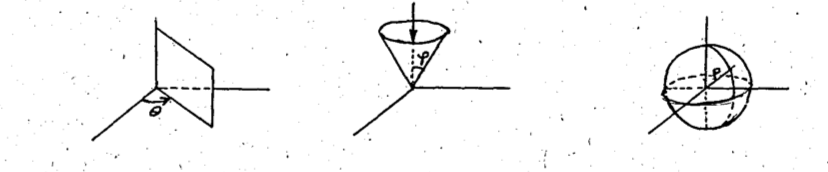
\includegraphics[width=\textwidth]{images/b2p1-200-1.png}


$\theta$-constant surface\quad\quad\quad\quad    
$\vartheta$-constant surface\quad\quad\quad\quad
$\rho$-constant surface\\

\quad\quad(a plane)       \quad\quad\quad\quad\quad\quad\quad\quad
(a cone)        \quad\quad\quad\quad\quad\quad\quad\quad
(a sphere)\\

We have one more set of transforming relations among three coordinate system which is between cylindrical and spherical one, namely
\begin{center}
\begin{multicols}{2}
\theta = \theta\\
r = \rho\sin\vartheta\\
z = \rho\cos\vartheta\\
\theta = \theta\\
\vartheta = \arctan\frac{r}{z}\\
\rho = \sqrt{r^{2} + z^{2}}\\

\end{multicols}
\end{center}

\begin{hEnumareteAlpha}
\item CYLINDERS, CONES, SURFACES OF REVOLUTION
\end{hEnumareteAlpha}
\begin{hEnumareteArabic}
\item Cylinders:
\end{hEnumareteArabic}
A surface S generated by a variable line $\ell$ of given direction $\Delta$, and subject to another condition such as intersecting a curve $\Gamma$ (or remaining tangent to a given surface $\Sigma$) is called a \underline{cylinder}.\\

\begin{multicols}{2}
The line $\ell$ is the \underline{generatix}, $\Delta$ the \underline{direction}, and $\Gamma$ the \underline{directix} of the cylinder $S$, and we say that $S$ in defined by $\Delta$ and $\Gamma$.\\
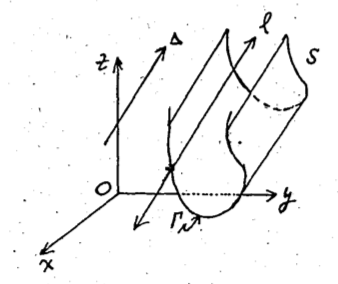
\includegraphics{images/b2p1-200-2.png}\\
\end{multicols}


\end{document}  

